\newcommand{\Treebeard}{{\sc {Treebeard}}}
\newcommand{\op}[1]{{\texttt {#1}}}

\section{Compiler Overview}
Figure \ref{Fig:CompilerStructure} shows the high level structure of Treebeard. 
The input to Treebeard is a serialized decision tree ensemble. Popular frameworks 
like XGBoost and LightGBM are supported and the system is easily extensible to other frameworks.
Given an input model our compiler generates optimized inference code. Specifically it generates a 
callable batch inference function \texttt{predictForest} that, given an array of input rows, computes an
array of model predictions. 
 
Treebeard specializes the code generated for inference by progressively optimizing and lowering a 
high level representation of the \texttt{predictForest} function down to LLVM IR \cite{LLVM}.
By \textbf{\emph{lowering}}, we mean the process of transforming an operation at a higher 
abstraction to a sequence of operations at a lower abstraction. Optimizations in Treebeard 
are implemented using a combination of annotation and lowering. An operation at a higher 
abstraction is annotated with attributes that indicate what kind of optimization is 
to be performed while lowering it. The lowering transformation uses this information to generate 
optimized lower level code. For example, tree tiling and loop order are decided 
at the highest abstraction. These decisions are communicated to the lowering pass 
which explicitly encodes them in the lowered IR as shown in figure \ref{Fig:Overview}.

%Treebeard first constructs a high level representation of the decision forest inference operation.
Treebeard's IR has three abstractions as shown in Figure \ref{Fig:Overview}.  
At the highest level (HIR), the input model is represented as a collection of binary trees. This is shown 
in the second row of figure \ref{Fig:Overview}. At this level of abstraction,
Treebeard tiles nodes together to transform a binary tree into an $n$-ary tree 
and decides what order trees are to be traversed in. In the example in the figure, 
trees are tiled with a tile size of 2. Tiling is indicated using colored elipses drawn 
around nodes that are in the same tile. Tree reordering is another transformation that is performed at this abstraction. 
One objective of tree reordering is to group identically structured trees so that they can share the same traversal code. 
With the tiling shown in Figure \ref{Fig:Overview}, Tree1 and Tree3 have depth 2, while Tree2 has a depth of 3.
Therefore, the trees are reordered so that Tree1 and Tree3 are together. 

The high level IR is then lowered to a mid-level IR (MIR). The aim of MIR is 
to allow optimizations that are independent of the final memory layout of the model. 
The lowering to MIR performs loop transformations like loop tiling, permutation, parallelization and unrolling.
At this level of the IR (the third row in Figure \ref{Fig:Overview}),
the order in which trees, input row pairs are walked is explicitly represented in the IR using loop nests.
Figure \ref{Fig:Overview} shows two possible ways that loop nests could be generated -- the first
walks all rows for one tree before moving to the next tree while the second walks all trees for 
one row before moving to the next row. Another aspect handled by this lowering is the fissing of 
loops to make sure that trees with the same structure share code. Here, both versions of MIR shown 
ensure that Tree1 and Tree3 share the same traversal code, while traversal code for Tree2 is different.
Additionally, tree walk optimizations, such as tree walk unrolling (shown in figure \ref{Fig:Overview}) and 
peeling are performed on the MIR.

Treebeard then further lowers the IR to explicitly represent the memory layout of the model. Buffers to hold model 
values are inserted into the generated code and all tree operations in the mid-level IR are lowered to explicitly 
reference these buffers. Additionally, at this level of the IR, Treebeard generates vectorized code to take 
advantage of SIMD instructions where applicable. Finally, the inference function is translated to LLVM IR and 
JIT compiled to executable code. 

%The following sections describe each level of the IR and their lowering in more detail.

\begin{figure}
  \centering
  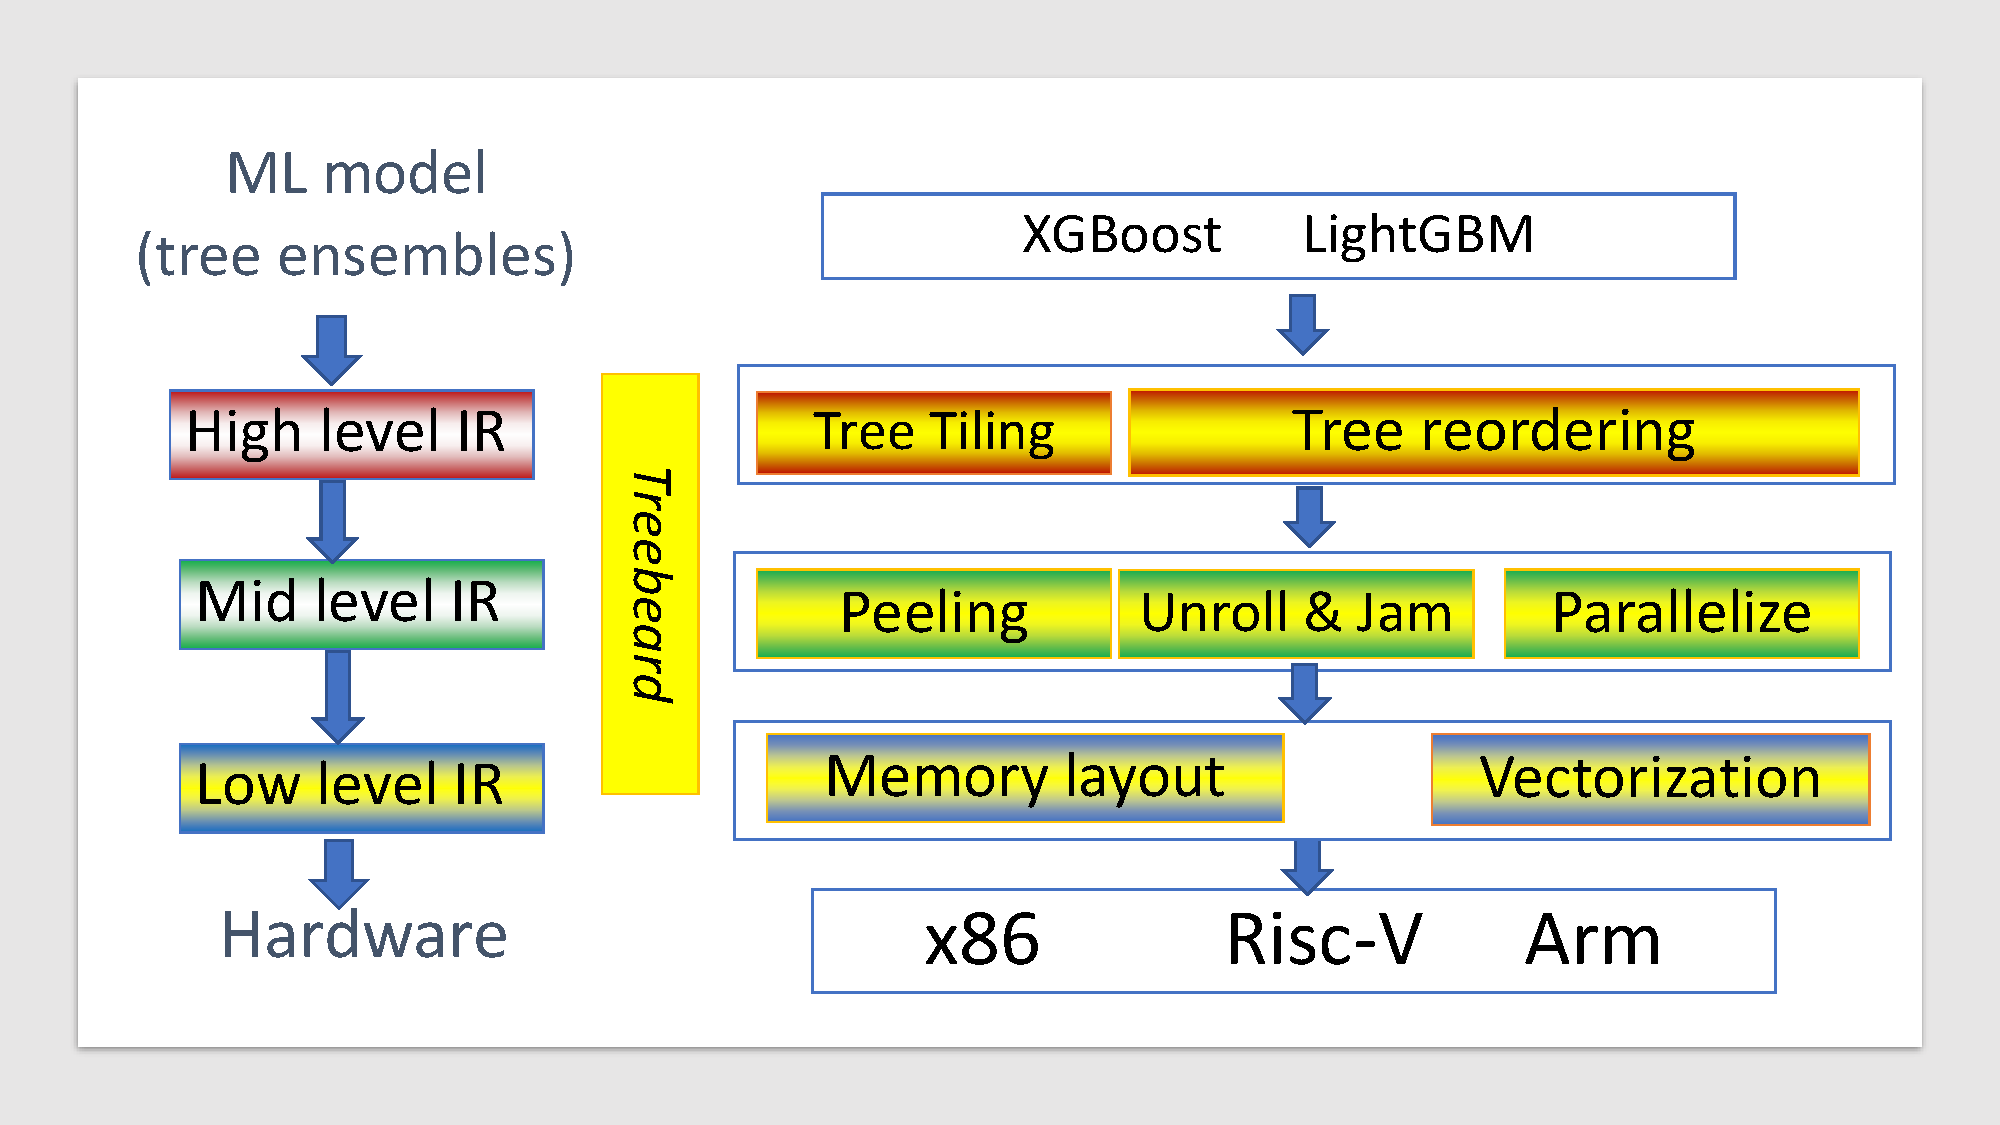
\includegraphics[width=\linewidth]{figures/compiler.pdf}
  \caption{Treebeard compiler structure}
  \label{Fig:CompilerStructure}
\end{figure}

\begin{figure*}
  \centering
  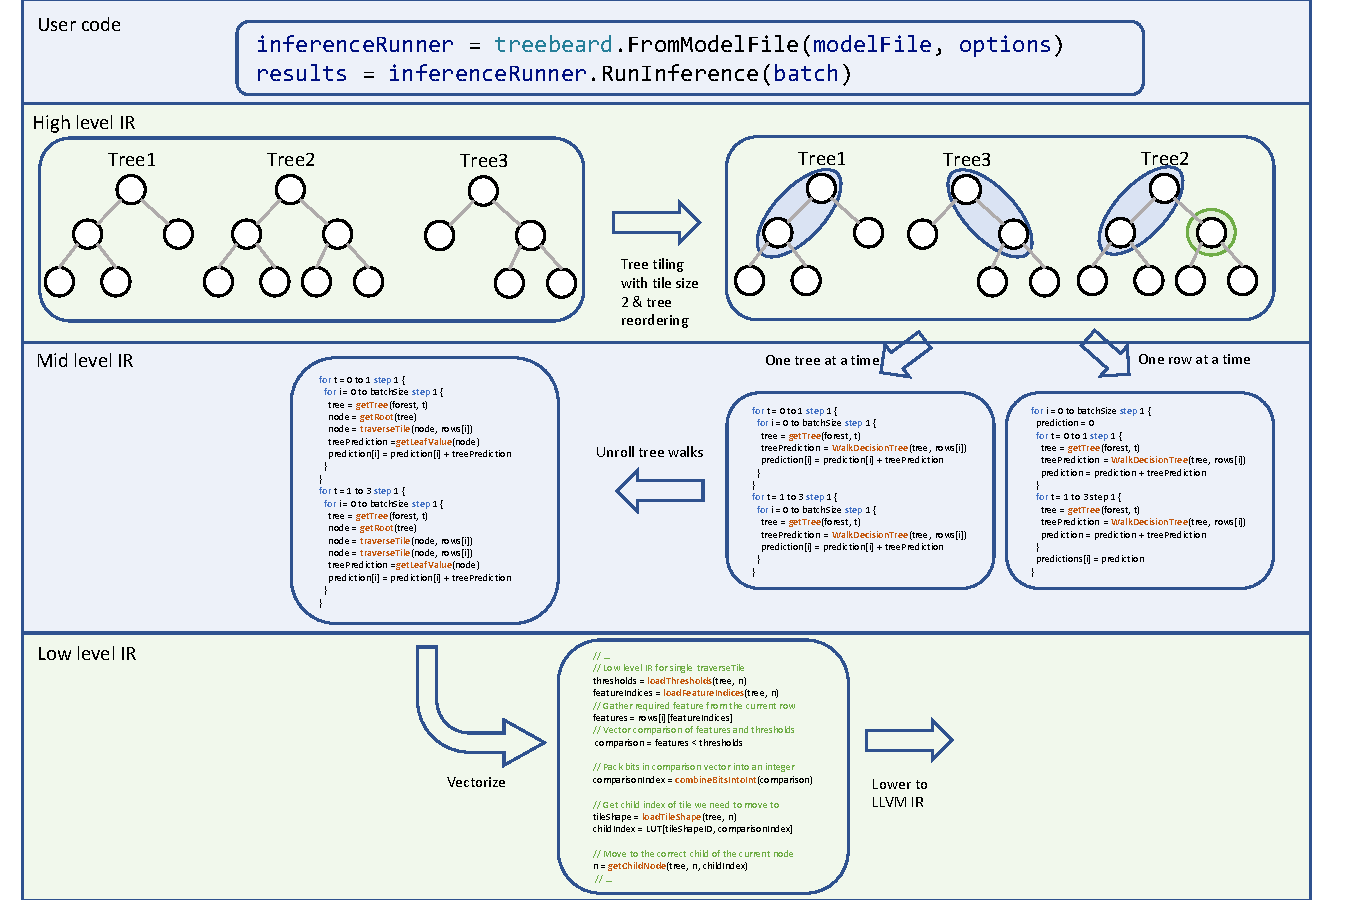
\includegraphics[width=\textwidth]{figures/OverviewExample.pdf}
  \caption{Treebeard IR lowering and optimization details. The three abstraction level in Treebeard's IR are shown. The
           high level IR is a tree based IR to perform model level optimization, the mid-level IR is for
           loop optimizations that are independent of memory layout and the low level IR allows us to perform
           vectorization and other memory layout dependent optimizations.}
  \label{Fig:Overview}
\end{figure*}



%\TODO{Should we describe the dialect's type system?}
% \TODO{Kr : consider focusing on the example instead of verbose description of optimizations. This section can be short, descriptions can come in later sections.}
% \subsection{High Level IR}
% As a first step Treebeard parses the input and generates a single MLIR operation, \texttt{predictForest} that represents inference using the input model on a set of rows. 
% At this level the operator simply contains a collection of binary trees. Two optimizations, tiling and tree ordering are applied at this level. The objective of tiling is to group nodes together so that the tree can be walked one tile at a time instead of one node at a time. We demonstrate that tiling can specialize the traversal of individual trees to either balance heavily skewed trees or proritize walks leading to higher probability leafs. Figure~\ref{ttile} shows examples of the tiling transformation. \TODO{kr: draw and explain example}. The objective of tree reordering is to group identically structured trees so that they can share the same traversal code. The predictForest function is now lowered to MIR with separate loop nests generated for traversing groups of identical trees. The generated MIR code is as shown below. 
% \TODO{show unoptimized loop nest as a listing}.

%The operation contains within it a tree based representation of the model that can be manipulated by optimizing transformations. Transformations on the model such as tiling, tree reordering and leaf padding are done at this level. The structure of the loop nest to walk the iteration space of trees and inputs is also decided at this level of the IR. \TODO{Should we mention that there is a scheduling language to decide this?}
% \begin{lstlisting}[language=C++]
% func Predict(float rows[batchSize]) {
%   predictions = predictForest(rows) 
%   return rows
% }
% \end{lstlisting}

% \subsection{Mid Level IR}
% The Mid Level IR optimizes the loop structures and tree walks. Firstly, the order in which the iteration space of trees and inputs is walked is determined and by re-ordering the loop nesting if necessary. Also, operations such as \texttt{isLeaf}, \texttt{traverseTile}, \texttt{getLeafValue} are introduced so that the traversal of trees explicitly represented. The following listing shows the IR for inference using a model with four trees on an input batch with two rows. The listed IR walks all trees for one input row before moving to the next row. One important point to note here is that details such as the data structure used for the trees are not explicitly encoded in the IR. This allows us to reuse optimization and lowering passes on this level of the IR regardless of what the final in memory representation of the model is.

% \begin{lstlisting}[style=c++]
%   // Constant that represents the model being compiled
%   forest = ensemble(...)
%   for i = 0 to 2 step 1 {
%     prediction = 0
%     for t = 0 to 4 step 1 {
%       tree = getTree(forest, t) 
%       node = getRoot(tree)
%       while (isLeaf(tree, n)==false)  do {
%         node = traverseTreeTile(tree, node, rows[i])
%       }
%       treePrediction = getLeafValue(tree, node)
%       prediction = prediction + treePrediction
%     }
%     predictions[i] = prediction
%   }
% \end{lstlisting}

% The IR listed above is a simplification of the actual IR. The actual IR is strongly typed and in SSA form.

% \subsection{Low Level IR}
% The IR is finally lowered to a form where the in memory representation of the model is made explicit. Buffers to hold the model values are inserted into the generated code and all tree operations in the mid-level IR are lowered to explicitly reference these buffers. The semantics of all operations are made explicit. For example, \texttt{traverseTreeTile} is lowered into a series of operations to load thresholds, feature indices and features, compare the features with the thresholds and compute the next node to evaluate. This IR is then lowered directly to LLVM IR and JITted.

